
\documentclass[11pt,border=1pt]{standalone}
\pdfcompresslevel=0\pdfobjcompresslevel=0 
%\usepackage[letterpaper]{geometry}
% amsmath package, useful for mathematical formulas
\usepackage{amsmath}
% amssymb package, useful for mathematical symbols
\usepackage{amssymb}
\usepackage{tikz}
\usepackage{graphicx}
\usepackage{relsize}
\usepackage{mathptmx}
\usetikzlibrary{matrix,positioning,arrows,fit,shapes,shadows,snakes,shadows}

% graphicx package, useful for including eps and pdf graphics
\usepackage{graphics,graphicx}

% Generate the pdf: latex Figure1;dvips Figure1.dvi;ps2epsi Figure1.ps;epspdf Figure1.epsi

%!TEX root = main_RNAPyro_JCB.tex

\newcommand{\ourprog}{\texttt{RNA-MoIP}\xspace} 

\usepackage[applemac]{inputenc} %for the encoding 


\newcommand{\RNAmutants}{\texttt{RNAmutants}\xspace}
\newcommand{\RNApyro}{\texttt{RNApyro}\xspace}

\newcommand{\red}[1]{{\color{red}#1}}
\newcommand{\farna}{\texttt{FARNA}\xspace}
\newcommand{\mcfoldmcsym}{\texttt{MC-Pipeline}\xspace}
\newcommand{\mcfold}{\texttt{MC-Fold}\xspace}
\newcommand{\mcsym}{\texttt{MC-Sym}\xspace}
\newcommand{\nast}{\texttt{NAST}\xspace}
\newcommand{\ifoldrna}{\texttt{iFoldRNA}\xspace}
\newcommand{\rnafold}{\texttt{RNAfold}\xspace}
\newcommand{\rnasubopt}{\texttt{RNAsubopt}\xspace}
\newcommand{\rnawolf}{\texttt{RNAwolf}\xspace}
\newcommand{\rnastructure}{\texttt{RNAstructure}\xspace}
\newcommand{\contrafold}{\texttt{contrafold}\xspace}
\newcommand{\unafold}{\texttt{unafold}\xspace}
\newcommand{\rnadd}{\texttt{RNA2D3D}\xspace}
\newcommand{\assemble}{\texttt{assemble}\xspace}
\newcommand{\fred}{\texttt{FR3D}\xspace}
\newcommand{\rnajunction}{\texttt{RNAjunction}\xspace}
\newcommand{\rnamotif}{\texttt{RNAmotif}\xspace}
\newcommand{\treefolder}{\texttt{TreeFolder}\xspace}
\newcommand{\barnacle}{\texttt{BARNACLE}\xspace}
\newcommand{\contextfold}{\texttt{contextfold}\xspace}
%\newcommand{\citep}{\cite}



\newcommand{\Z}[3]{\mathcal{Z}_{#1, #2}^{#3}}
\newcommand{\Y}[3]{\mathcal{Y}_{#1, #2}^{#3}}
\newcommand{\B}{\mathcal{B}}
\newcommand{\Kron}{\delta}

\newcommand{\ub}{\bullet}
\newcommand{\op}{\text{\tt(}}
\newcommand{\cp}{\text{\tt )}}

\newcommand{\Struct}{S}
\newcommand{\BoolFalse}{F}
\newcommand{\BoolTrue}{T}
\newcommand{\N}{{\sf N}}
\newcommand{\gc}{gc}

\newcommand{\PE}[1]{E(#1)}
\newcommand{\EI}{\text{EI}}
\newcommand{\ES}{\text{ES}}
\newcommand{\ISO}{\text{ISO}}

\newcommand{\EBP}[3]{E^{(#1)}_{{#2}\to{#3}}}


\newcommand{\Ab}{{\sf{A}}}
\newcommand{\Cb}{{\sf{C}}}
\newcommand{\Gb}{{\sf{G}}}
\newcommand{\Ub}{{\sf{U}}}


%%%%%%%%%%%% Comments macros %%%%%%%%%%%%%%%%%%%%%

\newcommand{\ShowTODO}[1]{{#1}}
\renewcommand{\ShowTODO}[1]{}

\newcommand{\TODO}[2]{\ShowTODO{\todo[inline, linecolor=#1, backgroundcolor=#1!60!white,bordercolor=#1]{#2}}}
\newcommand{\Discussion}[1]{\footnote{#1}}

\newcommand{\TODOTous}[1]{\TODO{orange}{{\bf TODO Tous :} #1}}
\newcommand{\TODOJerome}[1]{\TODO{blue!80!white}{{\bf TODO Jerome :} #1}}
\newcommand{\TODOYann}[1]{\TODO{gray}{{\bf TODO Yann :} #1}}
\newcommand{\TODOVlad}[1]{\TODO{green!60!black}{{\bf TODO Vlad :} #1}}

%%%%%%%%%%%%%%% End Comments %%%%%%%%%%%%%%%%%%%%%



\newcommand{\SpaceCheating}{\vspace{-0em}}
\newcommand{\ScaleDP}{.55}

\colorlet{StressColor}{red!60!black}

\pgfdeclarelayer{background}
\pgfsetlayers{background,main}

\begin{document}
\thispagestyle{empty}

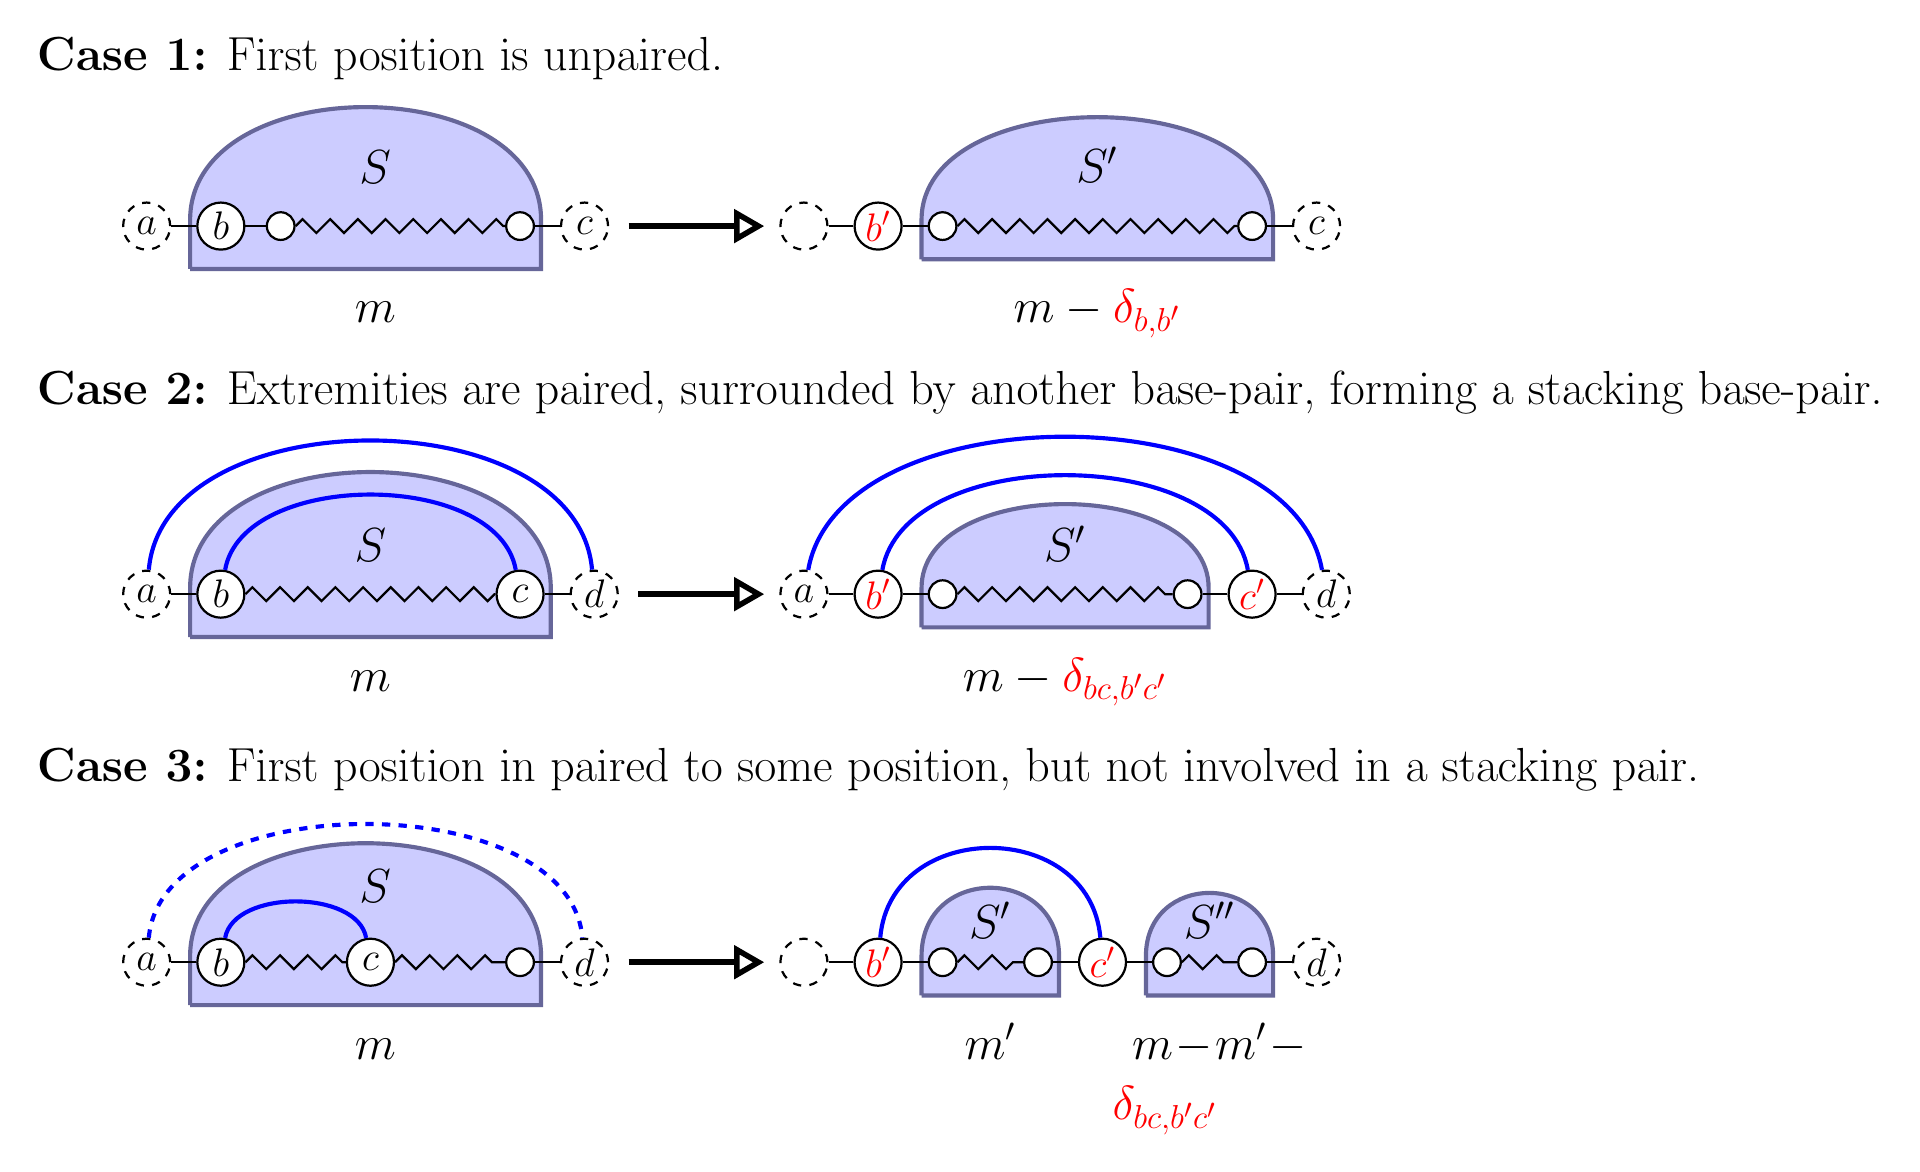
\begin{tikzpicture}[scale=.95]

  \newcommand{\BSep}{9pt}
  \newcommand{\HSep}{250pt}
  \newcommand{\VSepUp}{140pt}
  \newcommand{\VSepDown}{-140pt}
  \newcommand{\LabSepA}{63pt}
  \newcommand{\LabSepB}{75pt}
  \newcommand{\LabSepC}{72pt}
 
  \tikzstyle{base}=[circle,draw,thick,inner sep=0,minimum width=17pt,fill=white,,font={\relsize{+2}}]
  \tikzstyle{basesmall}=[circle,draw,thick,inner sep=0,minimum width=10pt,fill=white]
  \tikzstyle{basephantom}=[base,dashed,font=\relsize{+2}]
  \tikzstyle{linez}=[draw,snake=zigzag, segment aspect=.2,%
line after snake=0pt, 
        segment length=10pt,thick]
  \tikzstyle{lined}=[linez,draw,snake=none,thick]
  \tikzstyle{line}=[linez,draw,snake=none,thick]
  \tikzstyle{bp}=[in=95,out=85,draw,line width=1.5pt,blue,looseness=1]
  \tikzstyle{block}=[trapezium,trapezium angle=33, fill=blue!20, draw=blue!20!gray,line width=1.5pt, inner sep=0]
  \tikzstyle{lbl}=[inner sep=0]
  \tikzstyle{arr}=[line width=1.5pt,-open triangle 60,line width=2pt]
  \tikzstyle{caption}=[%fill=gray!20,draw=gray!60,thick,inner sep=4pt,rounded corners=6pt,
font=\relsize{+3},anchor=north west,xshift=-70pt]
  \tikzstyle{prob}=[fill=none,above=5pt,font=\relsize{+4},draw=none]
  \tikzstyle{cap2}=[fill=none,above=12pt,font=\relsize{+3}]





%% Inside part %%%%%%%%%%
{
%% Unpaired case %%%%%%%%%%

\begin{scope}[yshift=\VSepUp]
  \node[base] (a-1) at (0,0) {$b$};
  \node[basesmall] (a-1b) at (.8,0) {};
  \node[basesmall] (a-2) at (4,0) {};
  \node[left=\BSep of a-1, basephantom] (a-0) {$a$};
  \node[right=\BSep of a-2, basephantom] (a-3) {$c$}; 
  \node[right=0 of a-3] (x1) {};


  \path[lined] (a-1) --  (a-1b);
  \path[linez] (a-1b) --  (a-2);
  \path[lined] (a-0) -- (a-1);
  \path[lined] (a-2) -- (a-3);
  \node[lbl,below=3pt of a-1] (c1) {};
  \node[lbl,below=3pt of a-2] (c2) {};
  \path (a-1) --  node (xx1) {\phantom{xx3}} (a-2);

  \path[draw=none] (a-1) -- node[cap2] (s1) {$\Struct$}  (a-2);

  \begin{pgfonlayer}{background}
  \node[rectangle,inner sep=2pt,draw,fit=(a-1.west)(a-2.east) (c1) (c2)] (r1) {};
  \path[block]   (r1.south west) to (r1.south east) to (r1.north east) to[out=90,in=90,looseness=1.1] (r1.north west) to (r1.south west) ;
  \end{pgfonlayer}{background}
\end{scope}
\node[above= \LabSepA of a-1, caption] {{\bf Case 1:} First position is unpaired.};

\begin{scope}[xshift=\HSep,yshift=\VSepUp]
  \node[base] (a-1) at (0,0) {\color{red}$b'$};
  \node[basesmall,right=\BSep of a-1] (a-1b)  {};
  \node[basesmall] (a-2) at (5,0) {};
  \node[left=\BSep of a-1, basephantom] (a-0) {}; 
  \node[right=\BSep of a-2, basephantom] (a-3) {$c$};
  \path[linez] (a-1b) -- node (xy1) {} node[cap2] {$\Struct'$}  (a-2);
  \path[line] (a-1) -- (a-1b);
  \path[lined] (a-0) -- (a-1);
  \path[lined] (a-2) -- (a-3);
  \node[below=3pt of a-1b, inner sep=0] (c1) {};
  \node[below=3pt of a-2, inner sep=0] (c2) {};

  \node[xshift=-2pt] at (a-0.west) (y1) {};

\begin{pgfonlayer}{background}
  \node[rectangle,inner sep=2pt,draw,fit=(a-1b.west)(a-2.east) (c1) (c2)] (r1) {};
  \path[block]   (r1.south west) to  (r1.south east) to (r1.north east) to[out=90,in=90,looseness=1] (r1.north west) to (r1.south west) ;
  \end{pgfonlayer}{background}

\end{scope}

  \path (x1) edge[arr]    (y1);


%%%Stacking case %%%
\begin{scope}[yshift=0]
  \node[base] (a-1) at (0,0) {$b$};
  \node[base] (a-2) at (4,0) {$c$};


  \node[left=\BSep of a-1, basephantom] (a-0) {$a$};
  \node[right=\BSep of a-2, basephantom] (a-3) {$d$};
  \node[right=0 of a-3] (x2) {};

  \path[linez] (a-1) -- node (xx2) {} node[cap2,yshift=-4pt] (s2) {$\Struct$}  (a-2);

  \path[lined] (a-0) -- (a-1);
  \path[lined] (a-2) -- (a-3);
  \node[lbl,below=3pt of a-1] (c1) {};
  \node[lbl,below=3pt of a-2] (c2){};

  \draw[bp,looseness=1]  (a-0) to (a-3);
  \draw[bp,out=80,in=100,looseness=.9]  (a-1) to (a-2);
  \node[xshift=-2pt] at (a-0.west) (y3) {};

\begin{pgfonlayer}{background}
  \node[rectangle,inner sep=2pt,draw,fit=(a-1.west)(a-2.east) (c1) (c2)] (r1) {};
  \path[block]   (r1.south west) to   (r1.south east) to (r1.north east) to[out=90,in=90,looseness=1.1] (r1.north west) to (r1.south west) ;
  \end{pgfonlayer}{background}
\end{scope}
\node[above= \LabSepB of a-1, caption] {{\bf Case 2:} Extremities are paired, surrounded by another base-pair, forming a stacking base-pair.};

\begin{scope}[xshift=\HSep,yshift=00pt]
  \node[base] (a-1) at (0,0) {\color{red}$b'$};
  \node[base] (a-2) at (5,0) {\color{red}$c'$};

  \node[basesmall,right=\BSep of a-1] (a-1b) {};
  \node[basesmall,left=\BSep of a-2] (a-2b)  {};

  \node[left=\BSep of a-1, basephantom] (a-0) {$a$};
  \node[right=\BSep of a-2, basephantom] (a-3) {$d$};

  \path[linez] (a-1b) -- node (xy2) {}  node[cap2,yshift=-4pt]  {$\Struct'$}  (a-2b);

  \path[line] (a-1) -- (a-1b);
  \path[line] (a-2) -- (a-2b);
  \path[lined] (a-0) -- (a-1);
  \path[lined] (a-2) -- (a-3);
  \node[lbl,below=3pt of a-1b] (c1) {};
  \node[lbl,below=3pt of a-2b] (c2){};

  \draw[bp,out=80,in=100,looseness=.9]  (a-1) to (a-2);
  \draw[bp,out=80,in=100,looseness=.9]  (a-0) to (a-3);
  \node[xshift=-2pt] at (a-0.west) (y2) {};

\begin{pgfonlayer}{background}
  \node[rectangle,inner sep=2pt,draw,fit=(a-1b.west)(a-2b.east) (c1) (c2)] (r1) {};
  \path[block]   (r1.south west) to  (r1.south east) to (r1.north east) to[out=90,in=90,looseness=1] (r1.north west) to (r1.south west) ;
  \end{pgfonlayer}{background}
\end{scope}
 
  \path (x2) edge[arr] (y2);
%%% Junction case %%%%
\begin{scope}[yshift=\VSepDown] 
  \node[base] (a-1) at (0,0) {$b$};
  \node[basesmall] (a-2) at (4,0) {};
  \node[base] (a-2k) at (2,0) {$c$};

  \node[left=\BSep of a-1, basephantom] (a-0) {$a$};
  \node[right=\BSep of a-2, basephantom] (a-3) {$d$};
  \node[right=0 of a-3] (x3) {};


  \path[linez] (a-1) --  (a-2k);
  \path[linez] (a-2k) --  (a-2);
  \path[draw=none] (a-1) -- node[cap2,yshift=6pt](s3) {$\Struct$}  (a-2);

  \path (a-1) --  node (xx3) {} (a-2);


  \path[lined] (a-0) -- (a-1);
  \path[lined] (a-2) -- (a-3);
  \node[lbl,below=3pt of a-1] (c1) {};
  \node[lbl,below=3pt of a-2] (c2){};
  \node[lbl,below=3pt of a-2k] (c3){};

  \draw[bp,looseness=.9,dashed]  (a-0) to (a-3);
  \draw[bp,out=80,in=100,looseness=.9]  (a-1) to (a-2k);

\begin{pgfonlayer}{background}
  \node[rectangle,inner sep=2pt,draw,fit=(a-1.west)(a-2.east) (c1) (c2)] (r1) {};
  \path[block]   (r1.south west) to (r1.south east) to (r1.north east) to[out=90,in=90,looseness=1.1] (r1.north west) to (r1.south west) ;
  \end{pgfonlayer}{background}
\end{scope}

\node[above= \LabSepC of a-1, caption] {{\bf Case 3:} First position in paired to some position, but not involved in a stacking pair.};

\begin{scope}[xshift=\HSep,yshift=\VSepDown]
  \node[base] (a-1) at (0,0) {\color{red}$b'$};
  \node[base] (a-p) at (3,0) {\color{red}$c'$};

  \node[basesmall,right=\BSep of a-1] (a-1b) {};
  \node[basesmall,left=\BSep of a-p] (a-pb)  {};
  \node[basesmall,right=\BSep of a-p] (a-pa)  {};

  \node[basesmall] (a-2) at (5,0) {};
  \node[left=\BSep of a-1, basephantom] (a-0) {};
  \node[right=\BSep of a-2, basephantom] (a-3) {$d$};

  \path[linez] (a-1b) -- node (xy3) {} node[cap2,yshift=-7pt] {$\Struct'$} (a-pb);
  \path[linez] (a-pa) -- node (xz3) {} node[cap2,yshift=-7pt] {$\Struct''$} (a-2);

  \path[line] (a-1) -- (a-1b);
  \path[line] (a-pb) -- (a-p);
  \path[line] (a-pa) -- (a-p);

  \path[lined] (a-0) -- (a-1);
  \path[lined] (a-2) -- (a-3);
  \node[lbl,below=3pt of a-1b] (c1) {};
  \node[lbl,below=3pt of a-2] (c5){};
  \node[lbl,below=3pt of a-p] (c3) {};
  \node[lbl,below=3pt of a-pb] (c2){};
  \node[lbl,below=3pt of a-pa] (c4){};

  \draw[bp]  (a-1) to[looseness=1.4] (a-p);
  \node[xshift=-2pt] at (a-0.west) (y3) {};

\begin{pgfonlayer}{background}

  \node[rectangle,inner sep=2pt,draw,fit=(a-1b.west)(a-pb.east) (c1) (c2)] (r1) {};
  \path[block]   (r1.south west) to (r1.south east) to (r1.north east) to[out=90,in=90,looseness=1.7] (r1.north west) to (r1.south west) ; 

  \node[rectangle,inner sep=2pt,draw,fit=(a-pa.west)(a-2.east) (c4) (c5)] (r2) {};
  \path[block]   (r2.south west) to  (r2.south east) to (r2.north east) to[out=90,in=90,looseness=1.7] (r2.north west) to (r2.south west) ;

  \end{pgfonlayer}{background}

\end{scope}



  \path (x3) edge[arr] (y3);

 \newcommand{\CapSep}{35pt}
 \tikzstyle{cap3}=[anchor=base,font=\relsize{+3}] 

 \node[below=\CapSep of xx1.center,cap3] {$m$};
 \node[ below=\CapSep of xx2.center,cap3] {$m$};
 \node[ below=\CapSep of xx3.center,cap3] {$m$};

 \node[below=\CapSep of xy1.center,cap3] {$m-{\color{red}\Kron_{b,b'}}$};
 \node[below=\CapSep of xy2.center,cap3] {$m-{\color{red}\Kron_{bc,b'c'}}$};
 \node[below=\CapSep of xy3.center,cap3] {$m'$};
 \node[below=\CapSep of xz3.center,text width=7em,cap3] {\;\,$m-m'-{\color{red}\Kron_{bc,b'c'}}$

};

}

  
\end{tikzpicture}2
\end{document}